\subsection{Rust}

Rust ist eine compilierte system Programiersprache, welche trotz high level features hohe ausführungsgeschwindigkeiten verspricht. Anders als herkömmliche Programiersprachen verwendet Rust keinen Garbage Compiler, jedoch garantiert sie mit ihrem unkonventionellen Borrow Checker trotzdem Memory Safety.


Rust wurde 20xx von Person XX erfunden und in 20xx von Mozilla gesponsort\cite{rust}. In den letzten jahren verwenden immer mehr Entwickler, auch große firmen wie Google, Rust für ihre Projekte. Rust ist eine der am schnellsten wachsenden Programmiersprachen und hat sich in den letzten Jahren zu einer der beliebtesten System Programmiersprachen entwickelt \cite{stackoverflow_survey}.

\begin{figure}[ht]
  \centering
  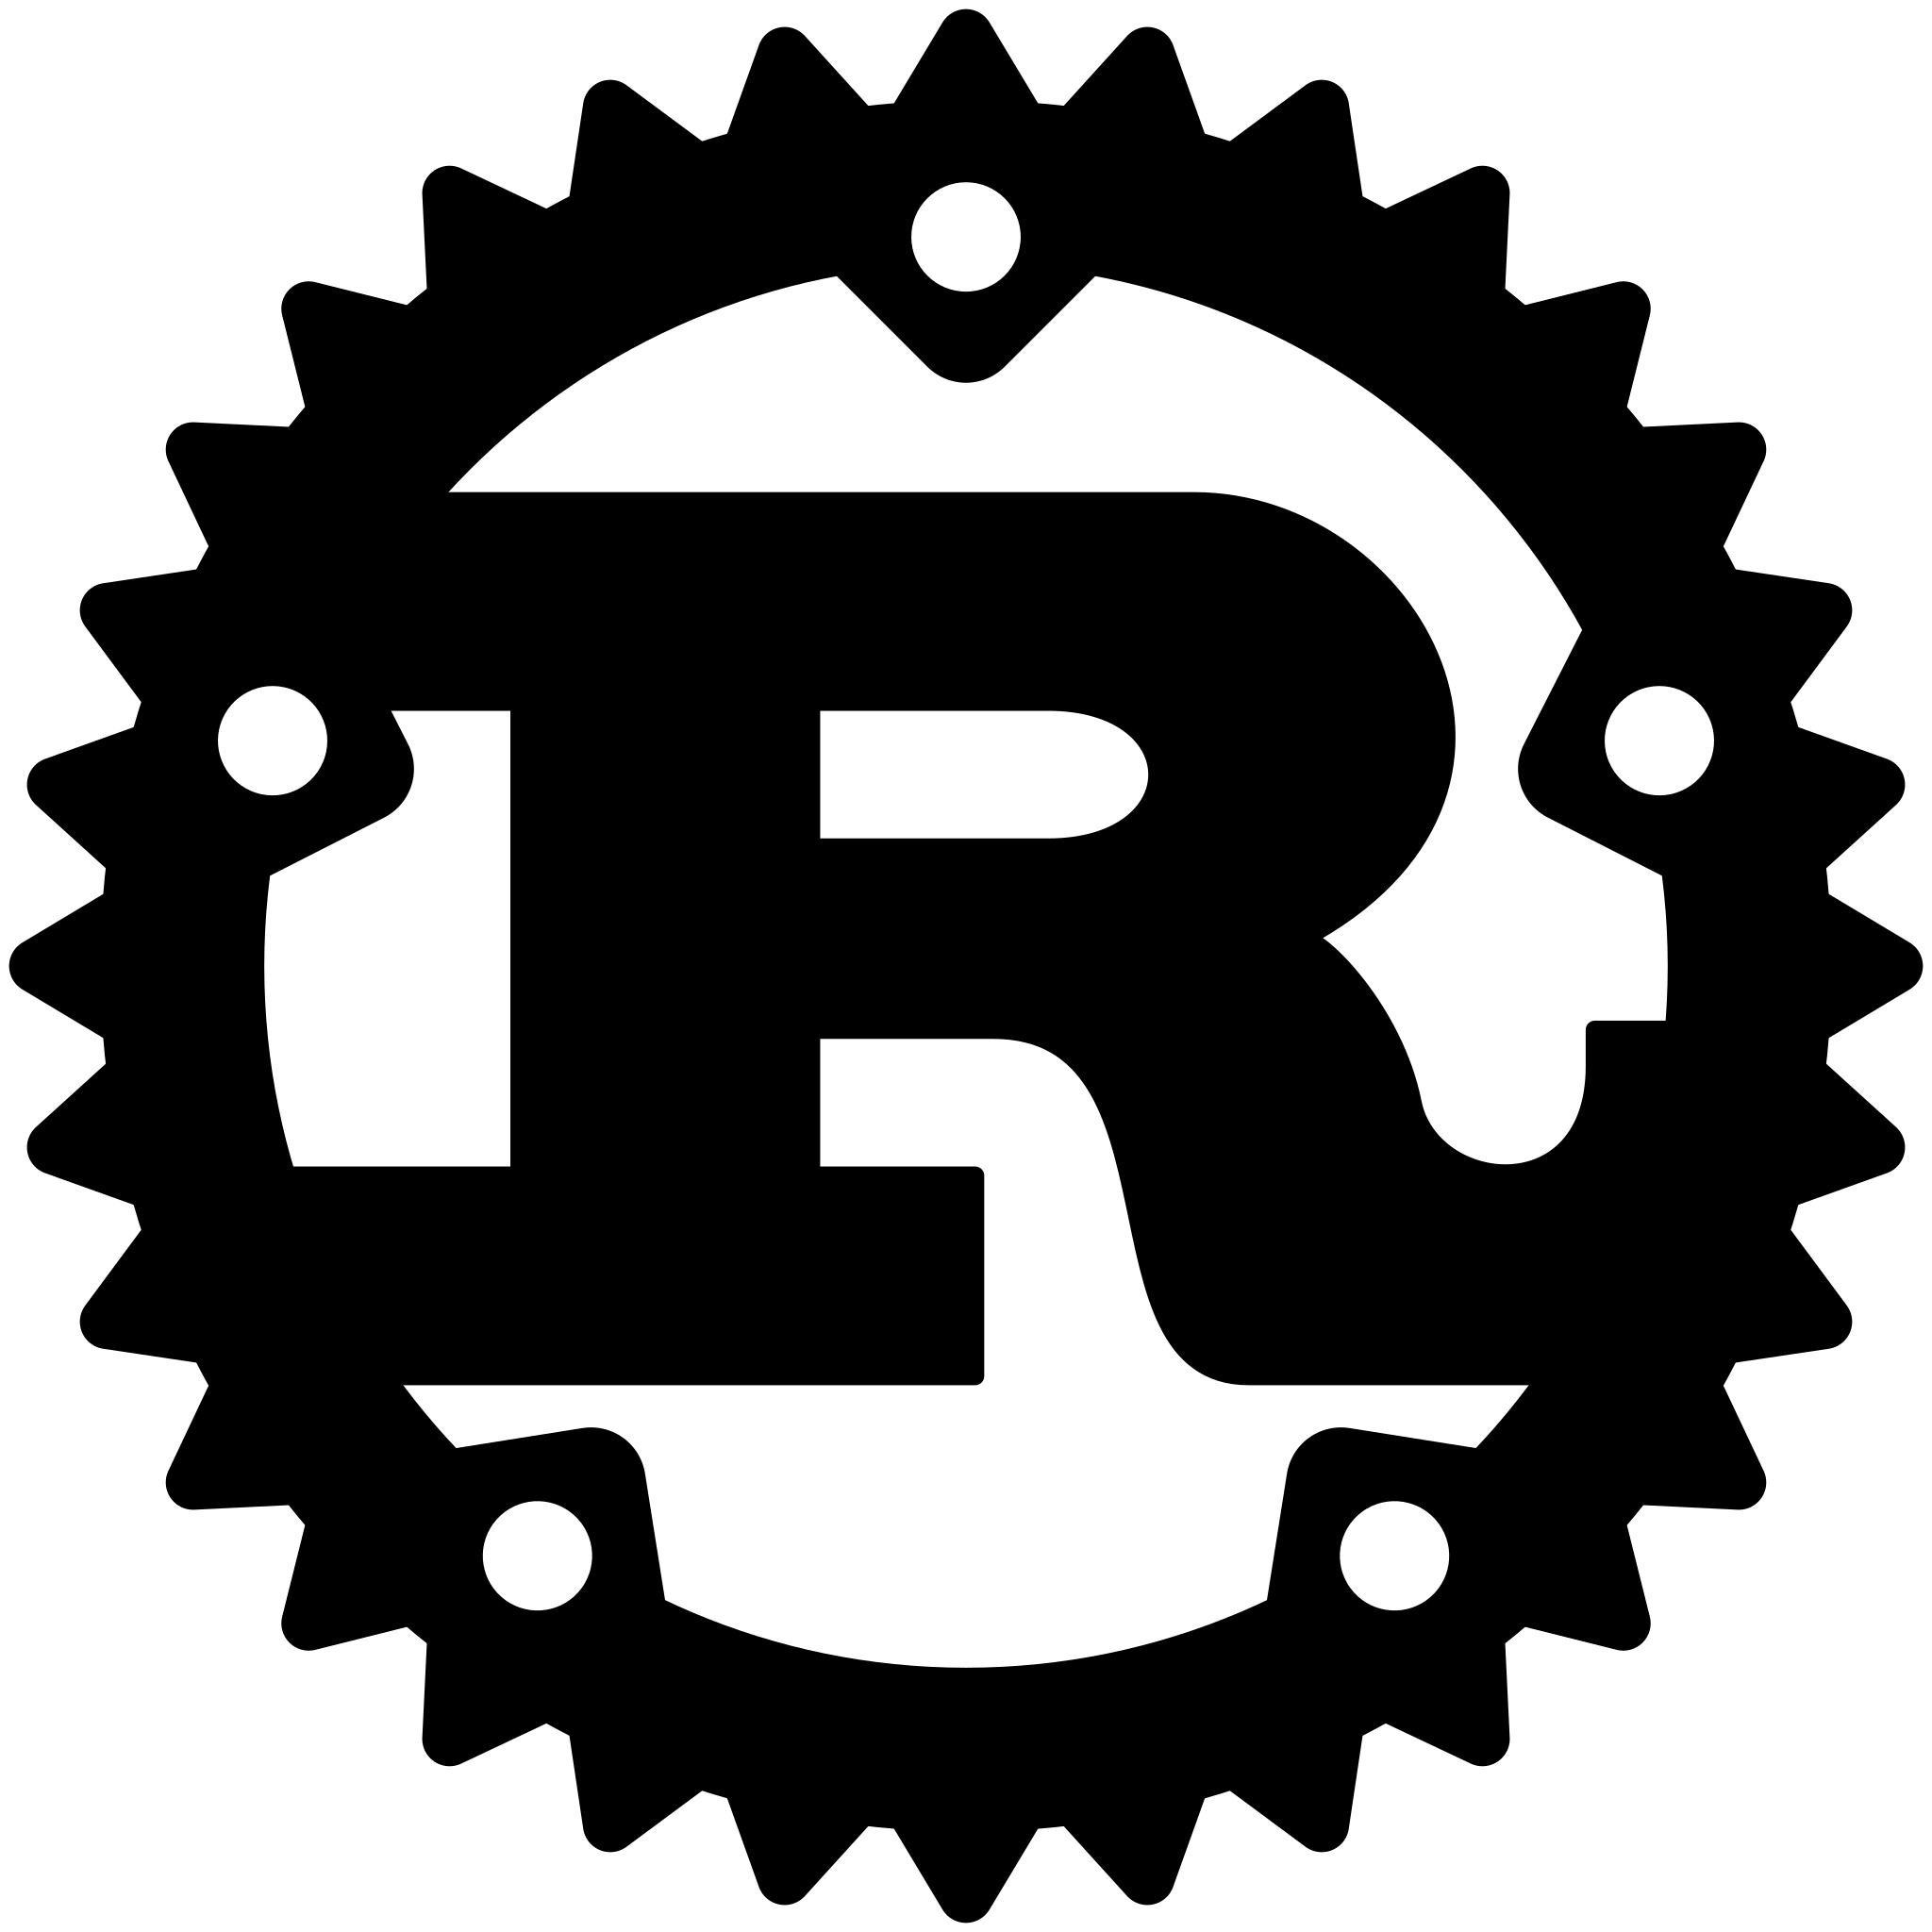
\includegraphics[width=0.20\textwidth]{images/rust_logo.png}
  \caption{Rust Logo}
  \label{fig:rust_logo}
\end{figure}

\subsubsection{firestore\_rs Softwarebibliothek}